
\chapter{Introduction}

\textit{Parts of this chapter have been published as J.\ Varennes, and A.\ Mugler, ``Sense and sensitivity: physical limits to multicellular sensing, migration, and drug response,'' Molecular pharmaceutics 13.7 (2016): 2224-2232.}
\vspace{5mm}

\noindent
Cells are extremely sensitive to their environment, capable of gathering information on chemicals in their environment with remarkable precision. For example, the amoeba \textit{Dictyostelium discoideum} is sensitive to chemical concentration differences on the order of ten molecules between its front and back half \cite{song2006dictyostelium}. Cell sensory precision of chemical concentrations is limited by the extrinsic noise inherent in molecule diffusion. The physical limits to concentration sensing due to extrinsic noise were theoretically derived 40 years ago by Berg and Purcell \cite{berg1977physics}, and it was shown that \textit{Escheria coli} bacteria operate very near the physical bound set by extrinsic noise \cite{lan2012energy}. Studies have revisited the topic of cell sensory precision to account for receptor binding kinetics, spatiotemporal correlations and spatial confinement
\cite{bialek2005physical, kaizu2014berg, bicknell2015limits}.

One very common cellular behavior in response to sensory information is chemotaxis and is defined as the process in which a cell or organism moves in response to a changing chemical concentration in its environment. Chemotaxis is critical to many biological processes in single-celled organisms as well as within multicellular organisms such as: nutrient search, organism development, wound healing, immune system targeting, and cancer metastasis \cite{iglesias2008navigating,roussos2011chemotaxis}.
One process that stands out for its significant impact on organism health is cancer metastasis. The first step of metastasis is invasion, wherein cells break away from their original tumor and invade the surrounding tissue. Our understanding of metastatic invasion has benefited tremendously from genetic and biochemical studies \cite{leber2009molecular, hanahan2000hallmarks, hanahan2011hallmarks}. However, the physical aspects of metastatic invasion are still unclear \cite{hanahan2011hallmarks}. Previous research shows that cancer cells sense and respond to chemical gradients provided by surrounding cells
\cite{bhowmick2004stromal, condeelis2006macrophages, shields2007autologous, puliafito2015three} as well as other features of the tumor environment
\cite{shields2007autologous, polacheck2011interstitial, shieh2011regulation} (Fig.\ \ref{fig:ch1_1}A,B). Indeed, cancer cells are extremely sensitive, able to detect a $1\%$ difference in concentration across the cell length
\cite{shields2007autologous}, and sometimes chemotax in response to these signals. Since metastasis is one of the most critical and lethal stages of cancer, studying the basic physics underlying chemotaxis can help us better understand metastasis.

There are two canonical forms of chemotaxis; cells either move towards the direction of increasing chemical concentration (positive chemotaxis), or they move away from the chemical and migrate in the direction of decreasing chemical concentration (negative chemotaxis). Positive chemotaxis may occur in response to nutrients in the environment, whereas negative chemotaxis is caused by waste or poisons in the environment that cells want to avoid. Analytical and computational models presented in this work are developed with respect to positive chemotaxis, though model conclusions are equally valid for the case of negative chemotaxis. We refer to the chemical signal that induces positive chemotaxis as the chemoattractant.

Chemotaxis can be viewed as a three step process: chemical sensing, polarization, and locomotion. In the presence of a sufficiently large chemical gradient a cell is able to detect a chemical concentration due to its receptors binding with the diffusing molecules in the environment. The gradient will result in more receptor binding events occurring on the side of the cell facing the higher concentration, and this difference causing an asymmetric response in the cell's internal sensory network. This leads to intracellular actin polymerization polarizing the cell along the asymmetry, and protrusions and retractions are made in the polarization direction \cite{jilkine2011comparison}. Due to the asymmetric distribution of protrusions the cell will preferentially move in the direction of polarization. Many studies have examined chemotaxis at the intracellular level in order to understand the biochemical machinery involved in producing polarization and locomotion \cite{petrie2009random}, but modeling how cell signaling produces polarization is still unclear \cite{iglesias2008navigating}.
Since chemical sensing is necessary for the initiation of chemotaxis, the extrinsic noise in the diffusing chemoattractant concentration affects chemotactic performance. Therefore studying the effect of extrinsic noise on chemotaxis can yield physical insight into chemotaxis and how it constrains the previously mentioned processes.


\begin{figure}[ht]
    \centering
        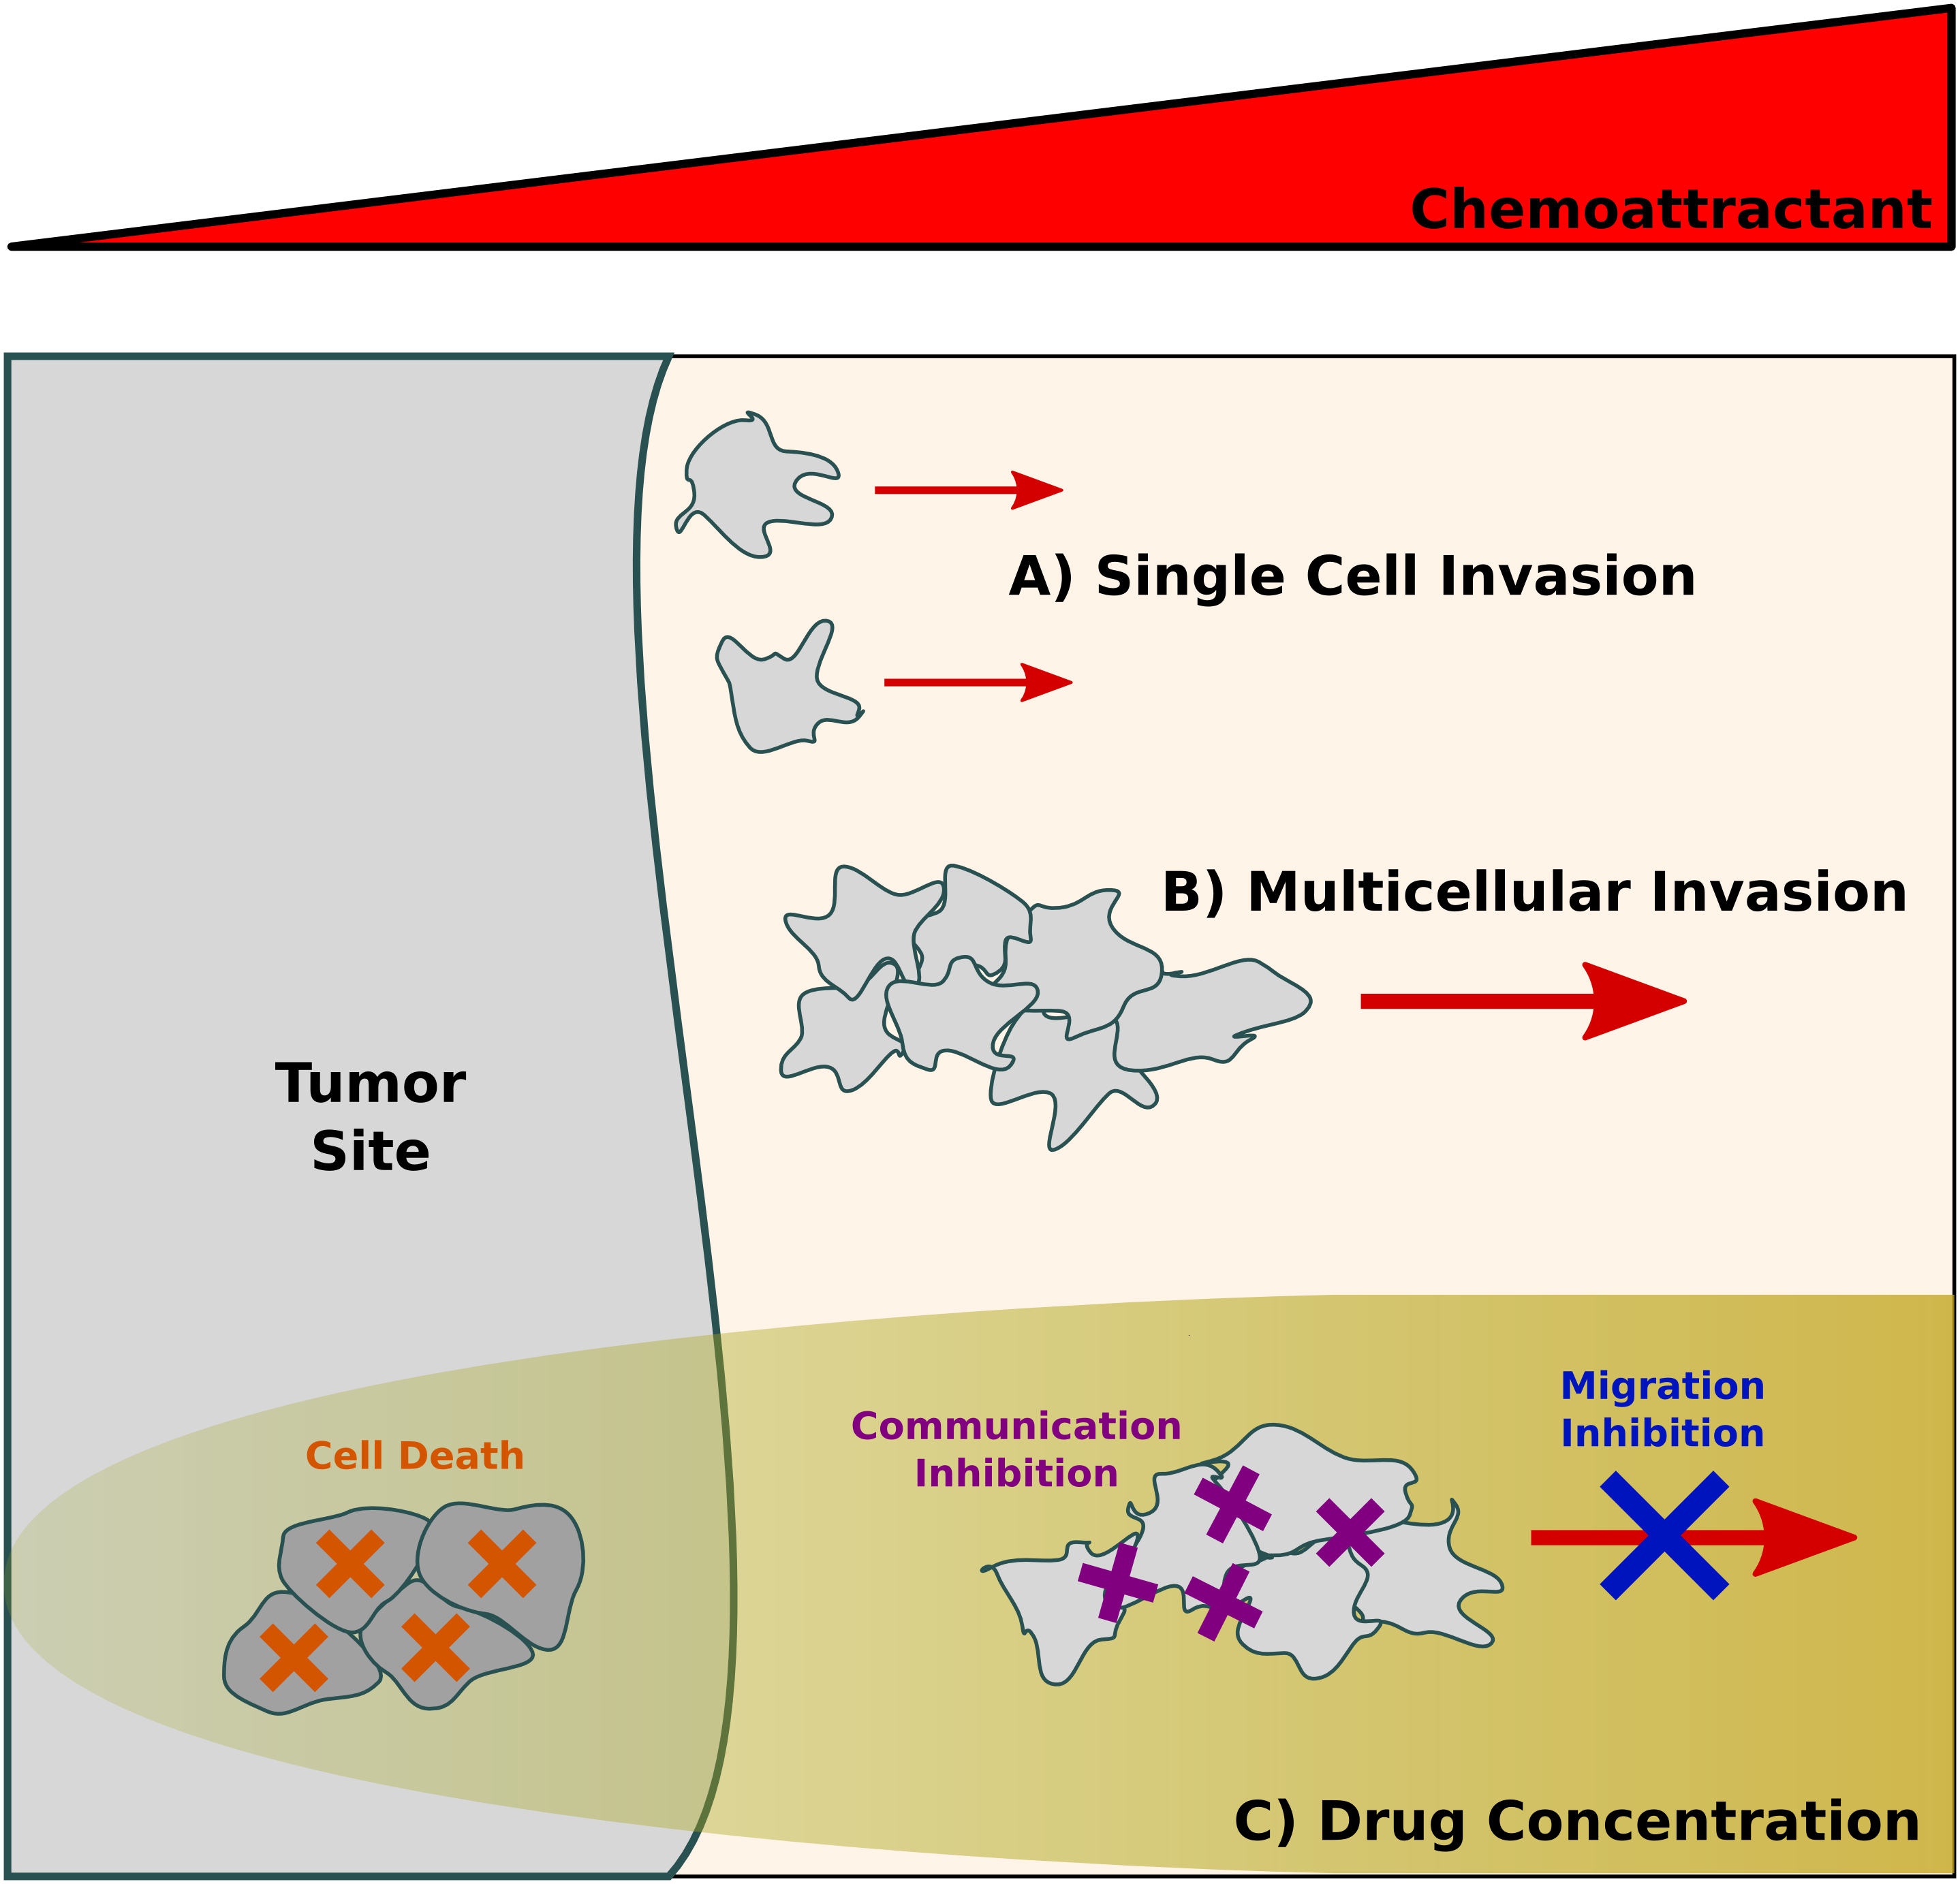
\includegraphics[width=0.8\textwidth]{../fig/ch1_fig1.png}
    \caption{Metastatic invasion is guided by chemical attractants and can occur via (A) single cells or (B) multicellular groups. (C) Drugs are delivered to the tumor environment in order to prevent tumor growth and metastasis. Drugs may cause cell death (orange), block cell-to-cell communication (purple), or prevent cell migration (blue).}
\label{fig:ch1_1}
\end{figure}


Furthermore, in many biological contexts cells act in close proximity to one another so their interactions may have a significant impact on their chemotactic performance \cite{theveneau2010collective}. During metastasis, chemotaxis can occur as a multicellular phenomenon involving the coherent motion of connected groups of cells (Fig.\ \ref{fig:ch1_1}B). In either the single-cell or multicellular case, the ability to precisely detect chemoattractants in the environment is bounded by the inherent diffusive fluctuations of the chemoattractants. Therefore it is important to understand the impact of diffusive noise on chemotactic precision.

In order to address the open question regarding how gradient sensing is linked to chemotactic performance we develop a framework of chemotaxis models. These theoretical and computational models
link sensing to polarization in order to examine how extrinsic noise from cell sensing puts physical constraints on chemotaxis. Starting in the following section, we briefly review the fundamental limits to concentration sensing and gradient sensing precision for single cells and multicellular collectives.
We also review how sensitive cells and collectives are to chemical signals and highlight how collective effects can enhance sensory response.
In Sect.\ 1.2 we review methods for modeling cell motion in relation to chemotaxis which will act as a foundation for the computational models developed in the proceeding chapters.

In Ch.\ 2 we review the physical limits to sensory precision, and discuss different chemotaxis modeling techniques.
Starting with Ch.\ 3, we apply computational and theoretical techniques to study human breast cancer cell chemotaxis. Computational simulations are conducted to explain and predict breast cancer cell chemotactic performance, and provide a relationship to common cell-migration experimental observables. We find that our simulations and theoretical model place physical constraints on the chemotactic performance of the cells observed in experiments. Single-cell chemotaxis simulations also give predictive power over how experimental parameters affect chemotactic performance in different ways.
Next, in Ch.\ 4 we examine multicellular chemotaxis. Cells very often exist and function in collective groups and chemotaxis is no different. We develop a novel theoretical approach to studying the effects of extrinsic noise on collective chemotaxis. We find that chemotactic performance is dependent on the type of collective behavior as well as on experimental parameters.
In Ch.\ 5 we extend our single-cell chemotaxis simulations to multicellular chemotaxis. We developed a model that explicitly accounts for the extrinsic noise in the diffusing chemoattractant concentration, as well as noise in intercellular communication in order to study the performance of communication-aided multicellular chemotaxis.
Finally, in Ch.\ 6 we summarize the models and results presented in the thesis.
